\documentclass[journal]{IEEEtran}
\usepackage{amsthm}
\usepackage{amsmath}
\usepackage{amssymb}
\usepackage{bbm}
\usepackage{algorithm}
\usepackage{algorithmic}
\usepackage{graphicx}
\newtheorem{theorem}{Theorem}
\newtheorem{definition}{Definition}
\newtheorem{corollary}{Corollary}
\newtheorem{proposition}{Proposition}
\newtheorem{lemma}{Lemma}
\newtheorem{remark}{Remark}
\newcommand{\A}{\frac{a \log(n)}{n}}
\newcommand{\B}{\frac{b \log(n)}{n}}
\newcommand{\cG}{\mathcal{G}}
\newcommand{\1}{\mathbbm{1}}
\DeclareMathOperator{\Var}{Var}
\DeclareMathOperator{\SSBM}{SSBM}
\DeclareMathOperator{\SIBM}{SIBM}
\DeclareMathOperator{\dist}{dist}

\title{Exact recovery of Stochastic Block Model by sampling from Ising model}
\author{
	Feng Zhao,~\IEEEmembership{Student Member, IEEE}\\
	Min Ye,~\IEEEmembership{Member, IEEE} and
	Shao-Lun~Huang,~\IEEEmembership{Member, IEEE}\\
	\thanks{Feng Zhao is with the
		Department of Electrical Engineering, Beijing, China.
		(Email: zhaof17@mails.tsinghua.edu.cn).
		Min Ye and S-L.~Huang are with the Data Science and Information
		Technology Research Center, Tsinghua-Berkeley Shenzhen Institute,
		Shenzhen, China (Email: \{yeemmi, shaolun.huang\}@sz.tsinghua.edu.cn).
	}}
	
\begin{document}
	\maketitle
\begin{abstract}
	Based on Ising model, we propose a stochastic algorithm to achieve the exact recovery for stochastic block model (SBM).
	The stochastic algorithm can be transformed to an optimization problem, which includes the special case of maximum likelihood.
	Besides, we give an unbiased convergent estimator for the parameters of SBM, which can be computed in constant time.
	Finally, we use metropolis sampling to realize the stochastic algorithm verify the error bound of our algorithm by experiments.
\end{abstract}
\begin{IEEEkeywords}
	stochastic block model, exact recovery, Ising model, modularity maximization, Metropolis sampling
\end{IEEEkeywords}
\section{Introduction}
Stochastic Block Model (SBM) is one of statistical modeling for community detection problems  \cite{holland1983stochastic, abbe2017community}.
It provides benchmark artificial dataset to evaluate different community detection algorithms.
Besides, SBM also inspires the design of algorithm for community detection tasks. These algorithms, such as
semi-definite relaxation, spectral clustering and label propagation, not only have theoretical guarantee when applied to SBM,
but perform well on dataset without SBM assumption. The study on the theoretical guarantee on SBM model can be divided between
the problem of exact recovery and that of partial recovery. For both cases, the asymptotic behavior of detection error
is analyzed when the scale of graph tends to infinity. There are already some well-known results of the exact recovery problem
on SBM.	To name but a few, Abbe and Mossel established the exact recovery region for a special sparse SBM with two communities  \cite{abbe2015exact, mossel2016}.
Later on, the result is extended to general SBM with multiple communities \cite{abbe2015community}.

Besides the recovery problem of SBM, inference of parameters on SBM provides a way to check whether the model fits the data well.
Previous inference methods require jointly estimation of node labels and model parameters \cite{nowicki2001estimation}, which have high complexity since the recovery and inference task are done simultaneously.
In this article, we will decouple the inference and recovery problem and propose an unbiased convergent estimator for SBM parameters when the number of communities is given. Once obtaining the estimator, the recovery condition can be checked to determine whether it is possible to recover the labels
exactly by other algorithms. Besides, the estimated parameter will guide the choice of parameters for our proposed stochastic algorithm.

Our analysis of maximal modularity is based on Ising model, which is a probability distribution of node states \cite{ising1925beitrag}.
Ising model is originally proposed in statistical mechanics to model the ferromagnetism phenomenon but has widely application in neuroscience, information theory
and social networks. Among different variants of Ising models, the phase transition property is shared. Based on the random graph generated by SBM with two underlining communities,
the Ising model is first studied by \cite{ye2020exact}. Our work will extend the existing result to multiple community case and establish the phase transition
property quantitatively by giving the recovery error upper bound. This error bound is polynomial decaying in two different phases respectively. Then we will propose a specialized Ising model using the definition of modularity. Sampling from this model,
we can achieve exact recovery for SBM.

Alternative to sampling from Ising model, we can find the state with maximal probability directly. This kind of method
is a generalization of maximum likelihood and also has connection with maximal modularity. Searching the state with maximal probability
could also be done within all balanced partition. We will show that the constrained search is equivalent with minimum cut problem and give the detection
error upper bound for both the unconstrained maximization and constrained one.

Exact solution to maximize the probability function or exact sampling from Ising model is NP hard. Many polynomial time algorithms have been proposed for approximation purpose.
Among these algorithms, simulated annealing performs well and produces a solution very close to the true maximal value \cite{liu2010detecting}.
On the other hand, in original Ising model,
metropolis sequential sampling is used to generate samples for Ising model \cite{metropolis1953equation}. Simulated annealing and metropolis sampling are closely related. In this article, we will
use metropolis sampling technique to sample from Ising model on SBM. This approximation enables us to verify the phase transition of our model property numerically.

This paper is organized as follows. Firstly, in section \ref{sec:psbm} we introduce SBM and give an estimator for the parameters of SBM.
Then in the next section \ref{sec:sibm}, the Ising model is given and quantitative description of its phase transition property is obtained.
Derived from the Ising model, in section \ref{sec:em}, we analyze the energy minimization method and establish its connection with maximum likelihood and modularity
maximization algorithm. Furthermore, in section \ref{sec:ms},
we realize the Ising model using metropolis algorithm to generate sample. Numerical experiments and conclusion are given at last to finish this paper.

Throughout this paper, the number of community is denoted by $k$; $m$ is the number of samples; $\lfloor x \rfloor$ is the floor function of $x$; the random undirected graph $G$ is written as $G(V,E)$ with vertex set $V$ and edge set $E$;
$V=\{1,\dots, n\} =: [n]$;
the label of each node is a random variable $X_i$; $X_i$ is chosen from $W= \{1, \omega, \dots, \omega^{k-1}\}$ and we further require $W$
is a cyclic group with order $k$; $W^n$ is the n-ary Cartesian power of $W$;
$f$ is a permutation function on $W$ and applied to $W^n$ in elementwise way;
the set $S_k$ is used to represent all permutation functions on $W$ and $S_k(\sigma):=\{f(\sigma)| f\in S_k\}$ for $\sigma \in W^n$;
the indicator function $\delta(x,y)$ is defined as
$\delta(x,y) = 1 $ when $x=y$, and $\delta(x,y)=0$ when $x\neq y$;
$g(n) = \Theta(f(n))$ if there exists constant $c_1 < c_2$ such that $c_1 f(n) \leq g(n) \leq c_2 f(n)$
for large $n$;
$\Lambda := \{ \omega^j  \cdot \mathbf{1}_n | j=0, \dots,k-1\}$
where $\mathbf{1}_n$ is the all one vector with dimension $n$;
we define the distance of two vectors as:
$\dist(\sigma, X)
=|\{i\in[n]:\sigma_i\neq X_i\}| \textrm{ for } \sigma,X\in W^n
$ and the distance of a vector to a space $S\subseteq W^n$
as
$\dist(\sigma,S)
:=\min\{\dist(\sigma, \sigma') | \sigma' \in S\}
$.
\section{Related Works}
The classical Ising model is defined on lattice and confined to two state $\{\pm 1\}$. This definition
can be extended to general graph and multiple state \cite{potts1952some}. In \cite{liu2017log}, Liu considered
the Ising model defined on graph generated by sparse SBM and his focus is to compute the log partition function,
which is averaged over the random graphs. In \cite{berthet2019exact}, an Ising model with repulsive interaction
is considered on a fixed graph structure, and the phase transition condition is established which involves both the assortative and disassortative
parameters. Our Ising model derives from the work of \cite{ye2020exact}, but we deepen the results by considering the error upper bound and
multiple community case.

The error upper bound for exact recovery of 2 community SBM by constrained maximum likelihood has been obtained in \cite{abbe2015exact}.
Using more careful analysis, we establish a sharper upper bound for multiple community case.
% our contribution and main results

\section{Stochastic Block Model and Parameter Estimation}\label{sec:psbm}
We consider a special symmetric stochastic block model, which is defined as follows:
	\begin{definition}[SSBM with $k$ communities] \label{def:SSBM}
	Let $0\leq q<p\leq 1$, $V=[n]$ and $X=(X_1,\dots,X_n)\in W^n$. $X$ satisfies the constraint that $|\{v \in [n] : X_v = u\}| = \frac{n}{k}$ for $u\in W$.
	The random graph $G$ is generated under $\SSBM(n,k,p,q)$ if
	\begin{enumerate}
	\item There is an edge of $G$ between the vertices $i$ and $j$ with probability $p$ if $X_i=X_j$ and with probability $q$ if $X_i \neq X_j$
	\item The existence of each edge is independent with each other.
	\end{enumerate}
\end{definition}
To explain SSBM in more detail,
we define the random variable $Z_{ij}:=\mathbbm{1}[\{i,j\} \in E(G)]$, which is the indicator function of the existence of an edge between node $i$ and $j$.
Given the node labels $X$, $Z_{ij}$ follows Bernoulli distribution, whose expectation is given by:
\begin{equation}
\mathbb{E}[Z_{ij}] =
\begin{cases}
p & \textrm{ if } X_i = X_j \\ 
q & \textrm{ if }  X_i \neq X_j
\end{cases}
\end{equation}
Then the random graph $G$ with $n$ nodes
is completely specified by $Z:=\{Z_{ij}, 1\leq i<j\leq n\}$ in which all $Z_{ij}$ are jointly independent.
The probability distribution for SBM can be written as:
\begin{align}
&P_G(Z = z| X) = p^{\sum_{X_i = X_j} z_{ij}}q^{\sum_{X_i \neq X_j} z_{ij}} \notag \\
&\quad \cdot (1-p)^{\sum_{X_i = X_j} (1-z_{ij})}(1-q)^{\sum_{X_i \neq X_j} (1-z_{ij})} \label{eq:GmL}
\end{align}
We will use the notation $\cG_n$ to represent the set containing all graphs with $n$ nodes. By the normalization property,
$P_G(\cG_n) = \sum_{G\in \cG_n}P_G(G)=1$.

In Definition \ref{def:SSBM}, we have supposed that the node label $X$ is given instead of uniformly distributed random variable
. Since maximum posterior estimator is equivalent to maximum likehood when the prior is uniform,
these two definitions are equivalent, and our assumption on $X$ make the following analysis more concise.

Given the SBM, the exact recovery problem can be formally defined as follows:
\begin{definition}[Exact recovery in SBM] \label{def:SSBMR}
Given $X$, the random graph $G$ is drawn under $\SSBM(n,k,p,q)$. If there exists an algorithm that takes
$G$ as input and outputs $\hat{X}$ such that
\begin{equation*}
P_a(\hat{X}):=P(\hat{X} \in S_k(X)) \to 1 \textrm{ as } n \to \infty
\end{equation*}
\end{definition}

In the above definition, the notation $P_a(\hat{X})$ is called the probability of accuracy for estimator $\hat{X}$.
Let $P_e(\hat{X}) = 1 - P_a(\hat{X})$ represent the probability of error. Definition \ref{def:SSBMR} can also
be formulated as $P_e(\hat{X}) \to 0$ as $n\to \infty$.
The notation $\hat{X} \in S_k(X)$ means that we can only
expect a recovery up to a global permutation of the ground truth label vector $X$. This is common in unsupervised
learning as no anchor exists to assign labels to different communities.
Besides, given a graph $G$, the algorithm can
be either deterministic or stochastic. The probability of $\hat{X} \in S_k(X)$ should be understood as 
$\sum_{G \in \cG_n} P_G(G) P_{\hat{X}|G}(\hat{X} \in S_k(X))$, which reduced to 
$P_G(\hat{X} \in S_k(X))$ for deterministic algorithm.

For constant $p,q$, that is, $p,q$ is irrelevant with the graph size $n$,
we can always find algorithms to recover $X$ such that the detection error decreases exponentially
fast with $n$.
That is to say, the task with dense graph is relatively easy to handle. Within this paper, we consider a sparse
case when $p = \A, q = \B$. This case corresponds to the sparsest graph when exact recovery of SBM is possible.
And under this condition, a well known result \cite{abbe2015community} states that
exact recovery is possible if and only if
\begin{equation}\label{eq:abk}
\sqrt{a} - \sqrt{b} > \sqrt{k}
\end{equation}

Before diving into the exact recovery problem, we first consider the inference problem for SBM.
Suppose $k$ is known and we want to estimate $a,b$ from the graph $G$.
Existing method needs to estimate the community structure and $a,b$ jointly. We give a simple method
by counting the number of edges $T_1$ and the number of triangles $T_2$ of $G$, and the estimators $\hat{a}, \hat{b}$ are
obtained by solving the following equation systems:
\begin{align}
\frac{x+(k-1)y}{2k} & = \frac{T_1}{n\log n} \label{eq:e_1}\\
\frac{1}{k^2}
\left(\frac{x^3}{6} + \frac{k-1}{2}xy^2 + (k-1)(k-2)\frac{y^3}{6}\right) & = \frac{T_2}{\log^3 n} \label{eq:e_2}
\end{align}
\begin{theorem}\label{thm:ab12}
When $n$ is large enough, the equation system \eqref{eq:e_1}, \eqref{eq:e_2} has unique solution $(\hat{a}, \hat{b})$,
which are unbiased consistent estimators
of $(a,b)$. That is,
$\mathbb{E}[\hat{a}] = a, \mathbb{E}[\hat{b}] = b$ and $\hat{a}, \hat{b}$ converges to $a,b$ in probability respectively.
\end{theorem}
Given a graph generated by SBM, we can use Theorem \ref{thm:ab12} to obtain the estimated $a,b$ and determine whether
exact recovery of label $X$ is possible by \eqref{eq:abk}.

Proof of Theorem \ref{thm:ab12} is postponed to Appendix and here we conduct a simple experiment to verify our conclusion.
We consider several combinations of $(a,b,k)$ and obtain the estimator $(\hat{a}, \hat{b})$, using
the empirical square error $\frac{1}{m} \sum_{i=1}^m (\hat{a}-a)^2 + (\hat{b}-b)^2$ as the criterion,
choosing $m=1000$ we obtain the following figure.
\begin{figure}[!ht]
	\centering
	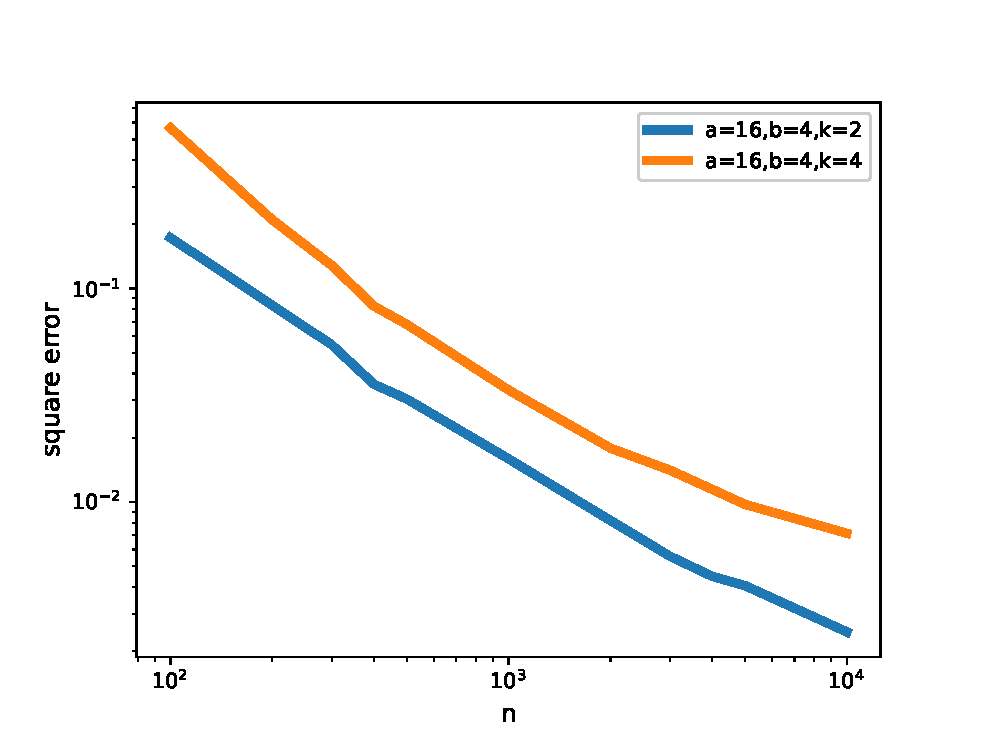
\includegraphics[width=0.45\textwidth]{estimator-error-2020-11-12.eps}
	\caption{estimation error with respect to $n$}
\end{figure}
From this figure we can see that as $n$ increases, MSE decreases polynomially fast. Therefore, the convergence
of $\hat{a} \to a$ and $\hat{b} \to b$ can be verified from this experiment.

\section{Ising model for Community Detection}\label{sec:sibm}
Now we have defined SBM and its exact recovery problem, the definition of Ising model on a graph genered by SBM is given
as follows:
\begin{definition}[Ising model with $k$ states]\label{def:ising}
	The Ising model on a graph $G$ sampled from $\SSBM(n,k,\A,\B)$ with parameters $\gamma,\beta>0$
	is a probability distribution on the configurations $\sigma\in W^n$ such that
	\begin{align} \label{eq:isingma}
	P_{\sigma|G}(\sigma=\bar{\sigma})=\frac{\exp(-\beta H(\bar{\sigma}))}{Z_G(\alpha,\beta)}
	\end{align}
	where
	\begin{equation}\label{eq:energy}
	H(\bar{\sigma}) = \gamma \frac{\log n}{n} \sum_{\{i,j\}\not\in E(G)} \delta(\bar{\sigma}_i, \bar{\sigma}_j)
	- \sum_{\{i,j\}\in E(G)} \delta(\bar{\sigma}_i, \bar{\sigma}_j)
	\end{equation}
	The subscript in $P_{\sigma|G}$ indicates that the distribution depends on $G$, and
	$Z_G(\alpha,\beta)$ is the normalizing constant for this distribution.
\end{definition}
In physics, we often call $\beta$ the inverse temperature and $Z_G(\gamma, \beta)$ the partition function.
The Hamiltonian energy $H(\bar{\sigma})$ consists of two terms: the repulsive interaction between nodes without edge connection
and the attractive interaction between nodes with edge connection. The term $\gamma$ is the ratio of the power of these two
interactions. We should add $\frac{\log n}{n}$ to balance the two terms because there are only $O(\frac{\log n}{n})$
connecting edges for each node.
The probability of each state is proportional to $\exp(-\beta H(\bar{\sigma}))$, and the state with the largest
probability corresponds to that with the lowest energy.

There are two main difference of Definition \ref{def:ising} with the classical one. Firstly we add a compulsory term
between nodes without an edge connection. This makes these nodes have larger probability to take different labels.
Secondly, we allow the state at each node to take $k$ values from $W$.
When $\gamma = 0$ and $k=2$, Definition \ref{def:ising}
reduces to the classical definition up to a scaling factor.

Definition \ref{def:ising} gives a stochastic estimator $\hat{X}^*$ for $X$. $\hat{X}^*$ is one sample generated from Ising model. The exact recovery error probability for $\hat{X}^*$ can be written as $P_e(\hat{X}^*) := \sum_{G \in \cG_n} P_G(G) P_{\sigma | G}(S^c_k(X))$. We can see from this expression that error probability is determined
by two parameters $(\gamma, \beta)$. When these parameters take proper value, $ P_e(\hat{X}^*)\to 0$ and the exact recovery of SBM is achievable. On the contrary, $P_e(\hat{X}^*) \to 1$ if $(\gamma, \beta)$ takes other values.
These two cases are summarized in the following theorem:
\begin{theorem}\label{thm:phase_transition}
Define the function $g(\beta), \tilde{g}(\beta)$ as follows:
\begin{equation}
g(\beta) = \frac{be^{\beta} + a e^{-\beta}}{k} - \frac{a+b}{k} +1
\end{equation}
and
\begin{equation}
\tilde{g}(\beta) = \begin{cases}
g(\beta) & \beta \leq \bar{\beta} = \frac{1}{2}\log \frac{a}{b} \\
g(\bar{\beta}) = 1 - \frac{(\sqrt{a} - \sqrt{b})^2}{k} & \beta > \bar{\beta}
\end{cases}
\end{equation}
where $\bar{\beta} =  \arg\min_{\beta > 0} g(\beta)$.
Let $\beta^*$ be defined as
$$
\beta^* = \log(\frac{a + b - k - \sqrt{(a + b - k)^2 - 4 a b)}}{2  b})
$$
which is the solution to the equation $g(\beta) = 0$ and $\beta^* < \bar{\beta}$. Then depending on
how $(\gamma, \beta)$ take values, $\forall \epsilon > 0$, when $n$ is sufficiently large, we have
\begin{enumerate}
\item If $\gamma > b$ and $\beta > \beta^*$,  $P_e(\hat{X}^*) \leq n^{\tilde{g}(\beta)/2 + \epsilon}$;
\item If $\gamma > b$ and $\beta < \beta^*$, $P_a(\hat{X}^*) \leq (1+o(1))\max\{n^{g(\bar{\beta})}, n^{-g(\beta) + \epsilon}\}$;
\item If $\gamma < b$, $P_a(\hat{X}^*) \leq \exp(-C n)$ for any $C>0$.
\end{enumerate}
\end{theorem}
By simple calculus, $\tilde{g}(\beta) < 0$ for $\beta> \beta^*$ and $g(\beta)>0$ for $\beta < \beta^*$.
For sufficiently small $\epsilon$ and as $n \to \infty$, the upper bound in Theorem \ref{thm:phase_transition} all converges to $0$ at least
in polynomial speed.
Therefore, Theorem \ref{thm:phase_transition} establishes the sharp phase transition property of SIBM model.
To illustrate Theorem
\ref{thm:phase_transition} more clearly,
let $D(\sigma, \sigma')$ be the event when $\sigma$ is nearest to $\sigma'$ among all its permutations.
That is
\begin{equation}
D(\sigma, \sigma') := \{ \sigma = \arg\min_{f \in S_k} \dist(f(\sigma), \sigma')  \}
\end{equation}
Then Theorem \ref{thm:phase_transition} can be stated in the following way:
\begin{corollary}\label{cor:phase4}
\begin{enumerate}
	\item If $\gamma > b$ and $\beta > \beta^*$, $P_{\SIBM}(\sigma = X | D(\sigma, X))  = 1-o(1)$;
	\item If $\gamma > b$ and $\beta < \beta^*$, $P_{\SIBM}(\sigma = X | D(\sigma, X))  = o(1)$;
\end{enumerate}	
\end{corollary}

The rest of this section is devoted to the proof of Theorem \ref{thm:phase_transition}, which relies on the
careful analysis on the one-flip energy difference. This useful result is summarized in the following lemma:
\begin{lemma}\label{lem:lemmaDiff}
	Suppose $\bar{\sigma}'$ differs from $\bar{\sigma}$ only at position $r$ by $\bar{\sigma}'_r = \omega^s \cdot \bar{\sigma}_r$.
	Then the change of energy is
	\begin{align}
	H(\bar{\sigma}') - H(\bar{\sigma}) &= (1+\gamma \frac{\log n}{n})\sum_{i \in N_r(G)} J_s(\bar{\sigma}_r, \bar{\sigma}_i)
	\notag \\
	&+ \gamma \frac{\log n}{n} (m(\omega^s \cdot \bar{\sigma}_r)-m(\bar{\sigma}_r)+1) \label{eq:DeltaH}
	\end{align}
	where $m(\omega^j) := |\{i \in [n] | \bar{\sigma}_i = \omega^j | \}$ and $J_s(x, y) = \delta(x, y) - \delta(\omega_s \cdot x, y)$
\end{lemma}
Lemma \ref{lem:lemmaDiff} gives an explicit way to compare the probability of two states by the following
equality:
\begin{equation}\label{eq:Pratio}
\frac{P_{\sigma |G } (\sigma = \bar{\sigma}')}{P_{\sigma |G } (\sigma = \bar{\sigma})}
= \exp(-\beta(H(\bar{\sigma}') - H(\bar{\sigma})))
\end{equation}
Besides, since the graph is sparse and every node has $O(\log n)$ neighbors, the computational cost (time complexity) for the energy difference
is also $O(\log n)$. 

When $H(\bar{\sigma}') < H(\bar{\sigma})$, we can expect $P_{\sigma | G}(\sigma = \bar{\sigma}')$ is far less than 
$P_{\sigma | G}(\sigma = \bar{\sigma})$. However,
since $G$ is sampled from SBM, the righthand side of \eqref{eq:Pratio} is a random variable. The proof of
Theorem \ref{thm:phase_transition} lies at the detailed analysis of the probabilistic property
of $ \exp(-\beta(H(\bar{\sigma}') - H(\bar{\sigma}))) $ and can be found in the Appendix.


\section{Community Detection via Energy Minimization}\label{sec:em}
Since $\beta^*$ is irrelevant with $n$, when $\gamma>b$, we can choose a sufficiently large $\beta$ such that
$\beta > \beta^*$, then by Theorem \ref{thm:phase_transition}, with almost 1 probability $\sigma \in S_k(X)$, which
implies that $P_{\sigma | G}(\sigma = X)$ has the largest probability for almost all graph $G$. Instead of generating
the sample from the Ising model, we can directly maximize the conditional probability to find this state with the largest probability.
Or equivalently, we can proceed by minimizing the energy term in \eqref{eq:energy}:
\begin{equation}\label{eq:hatX}
\hat{X}' := \arg\min_{\bar{\sigma} \in W^n} H(\bar{\sigma})
\end{equation}

In \eqref{eq:hatX}, we allow $\bar{\sigma}$ to take values from $W^n$. Since we know the ground truth label $X$ has equal
size $|\{v \in [n] : X_v = u\}| = \frac{n}{k}$, another formulation is to restrict the search space to
$W^*:= \{\sigma \big\vert |\{v \in [n] : \sigma_v = \omega^s\}| = \frac{n}{k}, s=0,1, \dots, k \}$.
When $\sigma \in W^*$, minimizing $H(\sigma)$ is equivalent to
\begin{equation}
\hat{X}'' = \min_{\sigma \in W^*} \sum_{\{i,j\} \not\in E(G) } \delta(\sigma_i, \sigma_j)
\end{equation}
which is the minimum cut between different detected communities.

When $\hat{X}'' \neq X'$, we must have $\dist(\hat{X}'' ,X)\geq 2$ to satisfy the constraint $\hat{X}'' \in W^*$.
Besides, the estimator of $\hat{X}''$ is parameter-free while $\hat{X}'$ depends on $\gamma$. The extra parameter $\gamma$ in the expression of
$\hat{X}'$ can be regarded as a kind of Lagrange multiplier for this integer programming problem. Thus the optimization problem for $\hat{X}'$
is a relaxation of that for $\hat{X}''$ by introducing a penalized term and enlarging the searched space from $W^*$ to $W$.

When $\beta > \bar{\beta}$, $\tilde{g}(\beta)$ becomes a constant value. Therefore, from Theorem \ref{thm:phase_transition} we can get that $n^{g(\bar{\beta})/2}$ is the fastest error rate upper bound for Ising estimator $\hat{X}^*$.
For the estimator $\hat{X}'$ and $\hat{X}''$, we can obtain sharper error upper bound, which is
summarized in the following theorem:
\begin{theorem}\label{thm:error_rate}
When $\sqrt{a} - \sqrt{b} > \sqrt{k}$, for $n$ sufficiently large, 
\begin{enumerate}
	\item if $\gamma > b$, $P_G(\hat{X}' \not\in S_k(X)) \leq (k-1+o(1))n^{g(\bar{\beta})}$;
	\item $P_G(\hat{X}'' \not\in S_k(X)) \leq ((k-1)^2+o(1))n^{2g(\bar{\beta})}$.
\end{enumerate}
\end{theorem}
As $g(\bar{\beta})<0$, $n^{2g(\bar{\beta})} < n^{g(\bar{\beta})} < n^{g(\bar{\beta})/2}$, then
Theorem \ref{thm:error_rate} implies that $P_e(\hat{X}'')$ has the sharpest upper bound among the three estimators.
This can be intuitively understood as the result of smaller search space.
The proof technique of Theorem \ref{thm:error_rate} is to consider the probability of events when $P_G(G | X) < P_G(G | \sigma)$
for $\dist(\sigma, X) \geq 1$. Then using union bound to sum them up.
This technique has been used in \cite{abbe2015exact} for $k=2$ to show exact recovery by maximum likelihood is possible
when $\sqrt{a} - \sqrt{b} > 2$ while a loose bound $n^{g(\bar{\beta})/4}$ is obtained.
For general case, since $\tilde{g}(\beta) = 1- \frac{(\sqrt{a} - \sqrt{b})^2}{k}$, Theorem \ref{thm:error_rate} implies that exact recovery is possible using $\hat{X}'$ as long as  
$\sqrt{a} - \sqrt{b} > \sqrt{k}$ is satisfied.


Estimator $\hat{X}'$ has one parameter $\gamma$. When $\gamma$ takes different values depending on $a,b$, $\hat{X}'$
is equivalent with maximum likelihood or maximum modularity in asymptotic case. The following analysis shows
such relationship intuitively.

Maximum likelihood estimator is obtained by maximizing the log likelihood function.
From \eqref{eq:GmL}, this function can be written as
$$
\log P_G(Z|X=\sigma) = -\log\frac{a}{b} \cdot H(\sigma) + C
$$
where $\gamma \frac{\log n}{n} = \frac{1}{\log(a/b)}(\log (1-\A) - \log (1-\B))$ and $C$ is a constant irrelevant with $\sigma$.
When $n$ is sufficiently large, we have $\gamma \to \gamma_{ML} := \frac{a-b}{\log(a/b)}$.
That is, maximum likelihood estimator is equivalent with $\hat{X}'$ when $\gamma = \gamma_{ML}$ asymptotically.


Maximum modularity estimator is obtained by maximizing the modularity of a graph, which is defined by
\begin{align}\label{eq:Q}
Q &= \frac{1}{2 |E|} \sum_{ij} (A_{ij} - \frac{d_i d_j}{2 |E|}) \delta(C_i, C_j)
\end{align}
where $d_i$ is the degree of the $i$-th node and $A$ is the adjacency matrix.
The modularity $Q$ can be re-written using the node label $\sigma$ as:
\begin{align}
Q(\sigma) = &-\sum_{\{i,j\} \not\in E(G) } \frac{d_i d_j}{2 |E|}\delta(\sigma_i,\sigma_j) \notag \\
&+ \sum_{\{i,j\} \in E(G) } (1 - \frac{d_i d_j}{2 |E|}) \delta(\sigma_i,\sigma_j)  \label{eq:Qtransform}
\end{align}
From \eqref{eq:Qtransform}, we can show that $Q(\sigma) \to -H(\sigma)$ with $\gamma = \gamma_{MQ} = \frac{a+b}{2}$ as $n\to \infty$.
Indeed, we have $d_i \sim \frac{\log n(a+b)}{2}, |E| \sim \frac{1}{2}n d_i$. Therefore, we have $\frac{d_id_j}{2|E|} \to \gamma_{MQ} \frac{\log n}{n} $. That is, maximum modularity estimator is equivalent with $\hat{X}'$ when $\gamma = \gamma_{MQ}$ asymptotically.


Using $a>b$ and the inequality $\log x > 2 \frac{x-1}{x+1}$ for $x>1$ we can verify that $\gamma_{MQ} > \gamma_{ML} > b$. That is, both maximum likelihood and maximum modularity satisfy the exact recovery conditions in Theorem \ref{thm:error_rate}.


\section{Community Detection based on Metropolis Sampling}\label{sec:ms}
From Theorem \ref{thm:phase_transition}, if we could sample from the Ising model, then with large probability, the sample
is aligned with $X$. However, the exact sampling is difficult when $n$ is very large since the cardinality of the state space increases in
the rate of $k^n$. Therefore, some approximation is
necessary. The most common way to generate an Ising sample is using Metropolis sampling \cite{metropolis1953equation}. 
Empirically speaking, starting from a random state, Metropolis algorithm updates the state by randomly selecting one position to flip at each iteration step.
Then after some initial burning time, the generated samples can be regarded as samples from Ising model.

The theoretical guarantee of Metropolis sampling is based on Markov chain. Under some general conditions, Metropolis samples are converging to
the steady state of the Markov chain, which is the probability distribution to be approximated. For Ising model, there is many previous works which have shown that the convergence of Metropolis sampling \cite{diaconis1998we}.

For our specific Ising model and energy term in \eqref{eq:energy},
the pseudo code of our algorithm is summarized in Algorithm \ref{alg:m}.
This algorithm requires the number of the communities $k$ to be known and the parameter $\gamma$ is given.
The iteration time $N$ should also be specified in advance.
\begin{algorithm}[H]
	\caption{Metropolis sampling algorithm for SBM} \label{alg:m}
	Inputs: the graph $G$, inverse temperature $\beta$, disassortative power $\gamma$ \\
	Output: $\hat{X}$
	\begin{algorithmic}[1]
		\STATE random initialize $\sigma \in W^n$
		\FOR{$i=1,2,\dots, N$}
		\STATE propose a new state $\bar{\sigma}'$ according to Lemma \ref{lem:lemmaDiff} where $s, r$ are randomly chosen
		\STATE compute $\Delta H(r,s) = H(\bar{\sigma}') - H(\bar{\sigma})$ using \eqref{eq:DeltaH}
		\IF{$\Delta H(r,s)<0$}
		\STATE $\sigma_r \leftarrow w^s \cdot \sigma_r$
		\ELSE
		\STATE with probability $\exp(-\beta \Delta H(r,s))$
			such that $\sigma_r \leftarrow w^s \cdot \sigma_r$
		\ENDIF
		\ENDFOR
	\end{algorithmic}
\end{algorithm}
The computation of $\Delta H(r,s)$ needs $O(\log n)$ time from Lemma \ref{lem:lemmaDiff}.
For some special Ising model with disassortative interaction, it needs to take $N=O(n\log n)$ to generate the sample for good approximation \cite{mcmc}. For our model, it is unknown whether $O(n\log n)$ is sufficient, and we empirically choose $N=O(n^2)$ in the experiments.
Then the time complexity of Algorithm \ref{alg:m} is $n^2 \log n$.

Using Metropolis sampling, we conduct a moderate simulation to verify Theorem \ref{thm:phase_transition}.
We choose $n=3200, k=2$, and the empirical accuracy is computed by $P_e = \frac{1}{m_1m_2}\sum_{i=1}^{m_1} \sum_{j=1}^{m_2} \mathbbm{1}[\hat{X}^* = \pm X]$. $m_1$ is the number of times to generate the random graph. For each $G$, we further sample $m_2$ states by Algorithm \ref{alg:m} consecutively.
To make good approximation, we choose $m_1=1000,m_2=5000$.
The result is shown in the following figure.
\begin{figure}[!ht]
	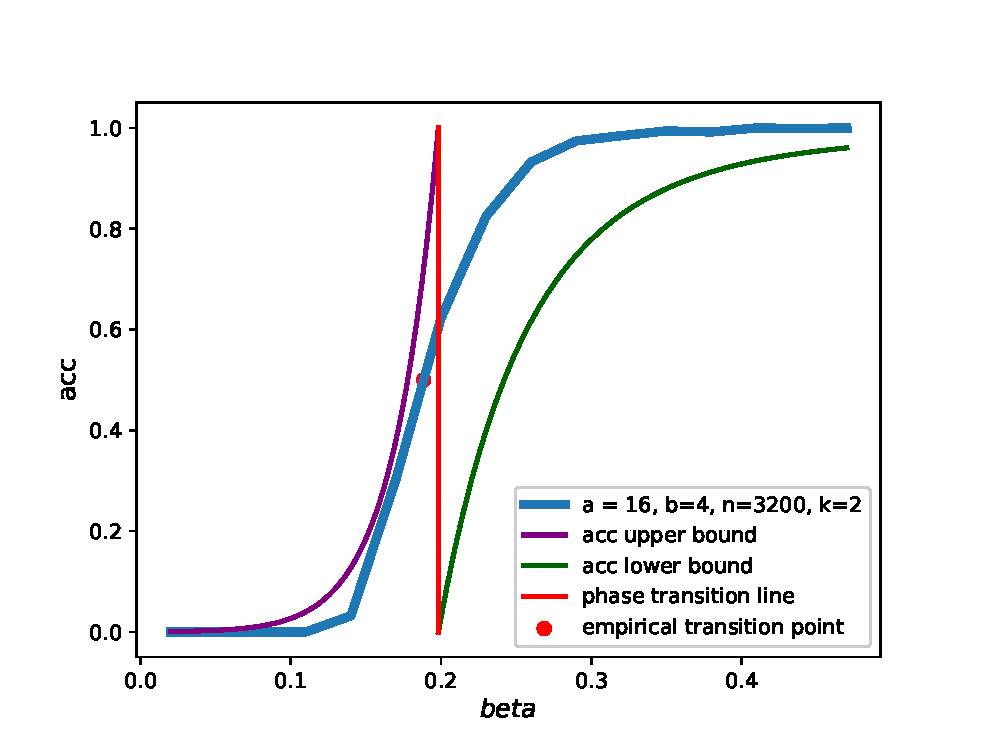
\includegraphics[width=0.45\textwidth]{beta_trans-2020-11-13.eps}
	\caption{the accuracy of exact recovery by SIBM}
\end{figure}

The vertical red line $\beta=0.2$ represents the phase transition threshold. The point $(0.19,0.5)$ in the figure
can be regarded as the empirical phase transition threshold, whose first coordinate is near to $\beta^* = 0.2$.
The green line $(\beta, n^{g(\beta)/2})$ is the theoretical lower bound of accuracy for $\beta>0.2$ while the orange line
$(\beta, n^{-g(\beta)})$ is the theoretical upper bound of accuracy for $\beta < 0.2$. It can be expected that
as $n$ is larger, the empirical accuracy curve (blue line in the figure) will approach the step function, which jumps from
0 to 1 at $\beta=0.2$.
\section{Conclusion}
In this paper, we have studies one convergent estimator (in Theorem \ref{thm:ab12}) to infer the parameters of SBM and three estimators to detect communities of SBM.
We give the exact recovery error upper bound for all the later three estimators (in Theorem \ref{thm:phase_transition}, \ref{thm:error_rate})
and study their connections. By introducing Ising model, our work breaks a new path to study the exact recovery problem for SBM. More
theoretical and empirical work will be done in the future such as the convergence of modularity (in \eqref{eq:Qtransform}) to the energy (in \eqref{eq:energy}), the necessary iteration time (in Algorithm \ref{alg:m}) for Metropolis sampling, and so on.
\appendix
\section*{Proof of Theorem \ref{thm:ab12}}
\begin{lemma}\label{lem:ER_tr_counting}
	Consider Erdos Renyi random graph $G$ with $n$ nodes, in which edges are placed independently with probability $p$ \cite{erdHos1960evolution}. Suppose
	$p=\A$, the number of edges is denoted by $|E|$ while the number of triangles is $T$. Then
	$\frac{|E|}{n \log n} \to \frac{a}{2}$ and $\frac{T}{\log^3 n} \to \frac{a^3}{6}$ in probability.
\end{lemma}
\begin{proof}
		Let $X_{ij}$ represents a Bernoulli random variable with parameter $p$. Then $|E| = \sum_{i,j} X_{ij}$, $X_{ij}$ are i.i.d.
	$E[T(G)] = \frac{n(n-1)}{2}p = \frac{(n-1)\log n}{2}a$ and $\Var[|E|] = \frac{n(n-1)}{2} p(1-p) < a\frac{(n-1)\log n}{2}$
	Then by Chebyshev's inequality
	\begin{align*}
	P(\Big|\frac{|E|}{n \log n } - \frac{a}{2} \frac{n-1}{n}\Big| > \epsilon) & \leq
	\frac{\Var[|E| /(n \log n )]}{\epsilon^2} \\
	& < \frac{a(n-1)}{2n^2\epsilon^2\log n}
	\end{align*}
	For a given $\epsilon$, when $n$ is sufficiently large,
	\begin{align*}
	P(\Big|\frac{|E|}{n \log n } - \frac{a}{2} \Big| > \epsilon) & <
	P(\Big|\frac{|E|}{n \log n } - \frac{a}{2} \frac{n-1}{n}\Big| > 2\epsilon) \\
	& \leq \frac{n-1}{8n^2 \epsilon^2 \log n}
	\end{align*}
	Therefore, by the definition of convergence in probability, we have $\frac{|E|}{n \log n} \to \frac{a}{2}$ as $n\to \infty$.
	
	Let $X_{ijk}$ represents a Bernoulli random variable with parameter $p^3$.
	Then $T = \sum_{i,j,k} X_{ijk}$.
	It is easy to compute that $E[T] = \binom{n}{3}p^3$. Since $X_{ijk}$ are not independent, the variance of $T$ needs careful calculation.
	From \cite{holland1977method} we know that
	% Mordern version: https://stats.stackexchange.com/questions/338267/distribution-and-variance-of-count-of-triangles-in-random-graph
	\begin{align*}
	\Var[T] & = \binom{n}{3} p^3 + 12 \binom{n}{4} p^5 + 30 \binom{n}{5} p^6 + 20 \binom{n}{6} p^6 - \binom{n}{3}^2 p^6 \\
	 & = O(\log^3 n)
	\end{align*}
	Therefore
	by Chebyshev's inequality
	\begin{align*}
	P(\Big|\frac{T}{\log^3 n } - \frac{a^3}{6} \frac{(n-1)(n-2)}{n^2}\Big| > \epsilon) &\leq \frac{\Var[T /\log^3 n ]}{\epsilon^2} \\ 
	& = \frac{1}{\epsilon^2}O(\frac{1}{\log^3 n})
	\end{align*}
	Hence, $\frac{T}{\log^3 n} \to \frac{a^3}{6}$.
\end{proof}
The convergence of $|E|$ in ER graph can be extended directly to SBM since the existence of each edge is independent.
But for $T$, it is a little tricky since the existence of each triangle is dependent with each other.  We need the following two lemmas
to proceed.
\begin{lemma}\label{lem:SBM_tr_counting_cross}
	Consider a 2 community SBM $(2n, p, q)$ and count the number of triangles $T$ which has a node in $S_1$ and an edge in $S_2$.
Then the variance of $T$ is
\begin{align}
\Var[T] & = \frac{n^2(n-1)}{2}q^2p + n^2(n-1)(n-2)p^2q^3 \notag \\
& + \frac{n^2(n-1)^2}{2}q^4p - \frac{n^2(n-1)(3n-4)}{2}q^4 p^2 \label{eq:SBM_tr_counting_cross}
\end{align}
\end{lemma}
\begin{lemma}\label{lem:SBM_tr_counting_3}
	Consider a 3 community SBM$(3n, p, q)$ and count the number of triangles $T$ which has a node in $S_1$, one node in $S_2$ and one node in $S_3$.
	Then the variance of $T$ is
	\begin{equation*}\label{eq:SBM_tr_counting_three}
	\Var[T] = q^3 n^3 + 3q^4 n^3(n-1) + 3q^5 n^3 (n-1)^2 - n^3(3n^2-3n+1)q^6
	\end{equation*}
\end{lemma}
The proof of the above two lemmas uses some counting techniques similar to that in \cite{holland1977method}, and we omit it here.
\begin{lemma}\label{lem:sbmV}
	For a SBM$(n, k, p, q)$ where $p=\frac{a\log n}{n}, q = \frac{b\log n}{n}$. The number of triangles is $T$.
	Then $\frac{T}{(\log n)^3}$ converges to $\frac{1}{k^2}(\frac{a^3}{6} + \frac{k-1}{2}ab^2 + (k-1)(k-2)\frac{b^3}{6} )$ in probability as $n \to \infty$.
\end{lemma}
\begin{proof}
	We split $T$ into three parts, the first is the number of triangles within community $i$, $T_i$. There are $k$ terms of $T_i$.
	The second is the number of triangles which have one node in community $i$ and one edge in community $j$, $T_{ij}$. There are $k(k-1)$ terms of $T_{ij}$. The third is the number of triangles which have one node in community $i$, one node in community $j$ and one node in community $k$.
	
	We only need to show that
	\begin{align}
	\frac{T_i}{\log ^3 n} &\to \frac{(a/k)^3}{6} \\
	\frac{T_{ij}}{\log^3 n}& \to \frac{1}{2}(a/k)(b/k)^2\\
	\frac{T_{ijk}}{\log^3 n} & \to (b/k)^3
	\end{align}
	The convergence of $\frac{T_i}{\log ^3 n}$ comes from Lemma \ref{lem:ER_tr_counting}.
	For $T_{ij}$ we use the conclusion from Lemma \ref{lem:SBM_tr_counting_cross}.
	We replace $n$ with $n/k$, $p=a\frac{\log n}{n}$, $q=b\frac{\log n}{n}$ in Equation \eqref{eq:SBM_tr_counting_cross}.
	$\Var[T_{ij}] \sim \frac{ab^2}{2k^3} \log^3 n$. Since the expectation of $\frac{T_{ij}}{\log^3 n}$ is $(n/k)\binom{n/k}{2}pq^2/(\log^3 n)
	=\frac{n-1}{n}\frac{ab^3}{k^3}$. By Chebyshev's inequality we can show that 
	\begin{align*}
	P( \Big|\frac{T_{ij}}{\log^3 n} - \frac{n-1}{n}\frac{ab^3}{k^3} \Big| > \epsilon) &\leq \frac{\Var[T_{ij} / \log^3 n]}{\epsilon^2} \\
	& = \frac{1}{\epsilon^2}
	O(\frac{1}{\log^3 n})
	\end{align*}
	Therefore, $\frac{T_{ij}}{\log^3 n} $ converges to $\frac{1}{2}(a/k)(b/k)^2$
	
	To prove $\frac{T_{ijk}}{\log^3 n}\to (b/k)^3$, from Lemma \ref{lem:SBM_tr_counting_3} we can get $\Var[T_{ijk}] = O(\log^5 n)$
	$$
	P( \Big|\frac{T_{ijk}}{\log^3 n} -\frac{b^3}{k^3} \Big| > \epsilon) \leq \frac{\Var[T_{ijk} / \log^3 n]}{\epsilon^2} = \frac{1}{\epsilon^2}
	O(\frac{1}{\log n})
	$$
\end{proof}
\begin{proof}[Proof of Theorem \ref{thm:ab12}]
	Let $e^*_1 = \frac{a+(k-1)b}{2k}$, $e^*_2 = \frac{a^3}{6} + \frac{k-1}{2}ab^2 + (k-1)(k-2)\frac{b^3}{6}$
	and $e_1 = \frac{T_1}{n\log n}, e_2 = \frac{T_2}{\log^3 n}$.
	From Lemma \ref{lem:ER_tr_counting}, $e_1 \to e^*_1$.
	From Lemma \ref{lem:sbmV}, $e_2 \to e^*_2$ as $n\to \infty$.
	Using $x=2ke_1 - (k-1)y$ we can get
\begin{equation}
g(y): = (k-1)(y^3 - 6 e_1 y^2 + 12 e_1^2 y) + 6 e_2 - 8 k e_1^3 = 0
\end{equation}
This equation has unique real root since $g(y)$ is increasing on $\mathbb{R}$:  $g'(y) = 3(k-1)(y-2e_1)^2 \geq 0 $.
Next we show the root lies within $(0, 2e_1)$.
\begin{align*}
\lim_{n\to \infty}g(0) &=  6e^*_2 - 8k(e^*_1)^3 =-\frac{3}{k^2}(k-1)(k-2)ab^2 \\
 &- \frac{k-1}{k^2} ((k-2)-(k-1)^2)b^3 < 0 \\
\lim_{n\to \infty}g(2e_1) &= 6e^*_2 - 8(e^*_1)^3 = \frac{(k-1)(a-b)^3}{k^3} > 0
\end{align*}

Therefore, we can get a unique solution $y$ within $(0, 2e_1)$. Since $(a,b)$ is a solution for the equation array. The conclusion follows.

By taking expectation on both sizes of \eqref{eq:e_1}, \eqref{eq:e_1} we can show $\mathbb{E}[\hat{a}] = a,
\mathbb{E}[\hat{b}] = b$. By the continuous property of $g(y)$, $\hat{b} \to b$ and $\hat{a} \to a$ follows similarly.
\end{proof}
\section*{Proof of Theorem \ref{thm:phase_transition}}
\begin{proof}[Proof of Lemma \ref{lem:lemmaDiff}]
	First we rewrite the energy term in \eqref{eq:energy} as:
	\begin{equation*}
	H(\bar{\sigma}) = \gamma \frac{\log n}{n} \sum_{i < j} \delta(\bar{\sigma}_i, \bar{\sigma}_j)
	- (1 + \gamma\frac{\log n}{n}) \sum_{ \{i, j\} \in E(G)} \delta(\bar{\sigma}_i, \bar{\sigma}_j)
	\end{equation*}
	Then calculating the energy difference term by:
	\begin{align*}
	H(\bar{\sigma}') - H(\bar{\sigma}) &= (1 + \gamma\frac{\log n}{n}) \\
	&\cdot \sum_{i \in N_r(G)} (\delta(\bar{\sigma}_r, \bar{\sigma}_i) -
	\delta(\omega^s \cdot \bar{\sigma}_r, \bar{\sigma}_i)) \\
	&+ \gamma \frac{\log n}{n}\sum_{i\neq r}
	( \delta(\omega^s \cdot \bar{\sigma}_r, \bar{\sigma}_i) -
	\delta( \bar{\sigma}_r, \bar{\sigma}_i) ) \\
	& = (1 + \gamma\frac{\log n}{n})\sum_{i \in N_r(G)} J_s(\bar{\sigma}_r, \bar{\sigma}_i) \\
	&+ \gamma \frac{\log n}{n}\sum_{i=1}^n
	( \delta(\omega^s \cdot \bar{\sigma}_r, \bar{\sigma}_i) -
	\delta( \bar{\sigma}_r, \bar{\sigma}_i) +1) \\
	&= (1+\gamma \frac{\log n}{n})\sum_{i \in N_r(G)} J_s(\bar{\sigma}_r, \bar{\sigma}_i)\\
	&+ \gamma \frac{\log n}{n} (m(\omega^s \cdot \bar{\sigma}_r)-m(\bar{\sigma}_r)+1)
	\end{align*}
\end{proof}
\begin{lemma}\label{lem:enhanced_fb}
	For $t\in [\frac{1}{k}(b-a), 0]$
	and $ r \le n/\sqrt{\log n}$
	\begin{equation} \label{eq:upmpt}
	\begin{aligned}
	& P_G(B_{\bar{\sigma}}-A_{\bar{\sigma}}\ge t r \log n)  \\
	\le & \exp\Big(r\log n
	\Big(f_{\beta}(t) - \beta t -1	+ O(\frac{1}{\sqrt{\log n}}) \Big)\Big) .
	\end{aligned}
	\end{equation}
\end{lemma}
Corresponding to the three cases of Theorem \ref{thm:phase_transition}, we use three non-trivial lemmas to 
establish the properties of Ising model.
\begin{lemma}\label{lem:sigmaX}
	Let $\gamma > b$. When $\dist(\bar{\sigma}, X) \geq \frac{n}{\sqrt{\log n}}$ and $\arg\,\min_{\sigma'\in S_k(X)} \dist(\bar{\sigma}, \sigma') = X$. The event
	$P_{\sigma | G}(\sigma = \bar{\sigma} ) > \exp(-Cn) P_{\sigma | G}(\sigma = X)$
	happens with probability (w.r.t. SSBM) less than $\exp(-\tau(\alpha,\beta) n \log^{1-\delta} n )$ where $C$ is an arbitrary constant, $\tau(\alpha,\beta)$ is a positive number.
\end{lemma}

\begin{lemma}\label{prop:small}
	If $\gamma>b$, $\beta>\beta^\ast$,
	For $1\leq r \leq \frac{n}{\sqrt{\log n}}$
	and $\forall \epsilon > 0$, there is a set $\cG^{(r)}$ such that
	\begin{equation}\label{eq:Gr}
	P_G(\cG^{(r)}_n) \ge 1 - n^{r(\tilde{g}(\beta)/2 + \epsilon)}
	\end{equation}
	and
	for every $G\in\cG^{(r)}_n$,
	\begin{equation}\label{eq:psigmaX}
	\frac{P_{\sigma|G}(\dist(\sigma, X)=r | D(\sigma, X))}
	{P_{\sigma|G}(\sigma=X | D(\sigma, X))} <
	n^{r \tilde{g}(\beta) /2}
	\end{equation}
	For $r> \frac{n}{\sqrt{\log n}}$, there is a set $\cG^{(r)}$ such that
	\begin{equation}\label{eq:Gr1}
	P(G\in\cG^{(r)}_n) \ge 1 - e^{-n}
	\end{equation}
	and
	for every $G\in\cG^{(r)}_n$,
	\begin{equation}\label{eq:psigmaX1}
	\frac{P_{\sigma|G}(\dist(\sigma, X)=r | D(\sigma, X))}
	{P_{\sigma|G}(\sigma=X | D(\sigma, X))} <
	e^{-n}
	\end{equation}
\end{lemma}


\begin{proof}
We distinguish the discussion between two cases: $r\leq \frac{n}{\sqrt{\log n}}$
and $r > \frac{n}{\sqrt{\log n}}$.
For $r=1$, taking $\bar{\sigma}=X$ in Lemma \ref{lem:lemmaDiff}, we have
\begin{equation}\label{eq:energy_diff}
H(\bar{\sigma}') - H(\bar{\sigma}) = (1+\gamma \frac{\log n}{n})(A^0_r - A^s_r) + \gamma\frac{\log n}{n}
\end{equation}
% Some additional notation is needed for the proof.
Similar with \eqref{eq:energy_diff}, generally we can write
$$
H(\bar{\sigma}) - H(X)=
(1 + \gamma \frac{ \log n}{n})[A_{\bar{\sigma}} - B_{\bar{\sigma}}] + \gamma\frac{ \log n}{n} N_{\bar{\sigma}}
$$
in which we use $A_{\bar{\sigma}}$ (or $B_{\bar{\sigma}}$) to represent the binomial random variable with parameter $\A$ (or $\B$)
respectively and $N_{\bar{\sigma}}$ is a deterministic positive number, irrelevant with the graph structure.

When $r\leq \frac{n}{\sqrt{\log n}}$, we can show that $\dist(\sigma, X) = r$ implies $D(\sigma, X)$ by using the triangle
inequality of $\dist$. For $f \in S_k \backslash \{ id \}$, we have
$$
\frac{2n}{k} \leq \dist(f(X), X) \leq \dist(\sigma, f(X)) + \dist(\sigma, X)
$$
Therefore, $\dist(\sigma, f(X)) \geq \frac{2n}{k} - \frac{n}{\sqrt{\log n}} \geq \dist(\sigma, X)$ and
\eqref{eq:psigmaX} is equivalent with
\begin{equation}\label{eq:psigmaX2}
\frac{P_{\sigma|G}(\dist(\sigma, X)=r)}
{P_{\sigma|G}(\sigma=X)} <
n^{r \tilde{g}(\beta) /2}
\end{equation}
The left hand side can be written as:
\begin{align*}
\frac{P_{\sigma|G}(\dist(\sigma, X)=r)}
{P_{\sigma|G}(\sigma=X)}  &= \sum_{\dist(\bar{\sigma}, X)=r}\exp(-\beta(H(\bar{\sigma})-H(X)))\\
&\leq \sum_{\dist(\bar{\sigma}, X)=r}\exp(\beta_n(B_{\bar{\sigma}}-A_{\bar{\sigma}}))
\end{align*}


Define $\Xi_n(r): = \sum_{\dist(\bar{\sigma}, X)=r}\exp(\beta_n(B_{\bar{\sigma}}-A_{\bar{\sigma}}))$ and we only need to show that
\begin{equation}
P_{G}(\Xi_n(r) \geq n^{r \tilde{g}(\beta) /2}) \leq  n^{r (\tilde{g}(\beta) /2 + \epsilon)}
\end{equation}
Define the event $\Lambda_n(G,r):=\{B_{\bar{\sigma}} -A_{\bar{\sigma}} < 0, \forall \dist(\bar{\sigma}, X)=r\}$,
we proceed as follows:
\begin{align*}
P_{G}(\Xi_n(r) \geq n^{r \tilde{g}(\beta) /2}) &\leq
P_G(\Lambda_n(G,r)^c) \\
&+ P_G(\Xi_n(r) \geq n^{r \tilde{g}(\beta) /2} |\Lambda_n(G,r) )
\end{align*}
For the first term, 
$P_G(\Lambda_n(G,r)^c) \leq n^{rg(\bar{\beta})} \leq n^{r (\tilde{g}(\beta) /2 + \epsilon/2)}$.
For the second term, we use Markov inequality:
\begin{align*}
P_G(\Xi_n(r) \geq n^{r \tilde{g}(\beta) /2} |\Lambda_n(G,r) )
\leq \mathbb{E}[\Xi_n(r)|\Lambda_n(G,r)]n^{-r \tilde{g}(\beta) /2} 
\end{align*}
The conditional expectation can be estimated as follows:
\begin{align*}
&\mathbb{E}[\Xi_n(r)|\Lambda_n(G,r)]=
\sum_{\dist(\bar{\sigma}, X) = r}\sum_{tr\log n = -\infty }^{-1} \\
& P_G(B_{\bar{\sigma}} -A_{\bar{\sigma}}=tr\log n)\exp(\beta_n tr \log n) \\
& \leq (k-1)^r n^{r+r\beta(b-a)/k} +
\sum_{\dist(\bar{\sigma}, X) = r}\sum_{tr\log n = r(b-a)/k\log n }^{-1} \\
& P_G(B_{\bar{\sigma}} -A_{\bar{\sigma}}=t\log n)\exp(\beta_n rt \log n)
\end{align*}
$r+r\beta(b-a)/k = f_{\beta}(\frac{b-a}{k}) < \tilde{g}(\beta)$, therefore,
$(k-1)^r n^{r+r\beta(b-a)/k}n^{-r \tilde{g}(\beta) /2} \leq n^{r (\tilde{g}(\beta) /2 + \epsilon/2)} $.
Using Lemma \ref{lem:enhanced_fb}, we have
\begin{align*}
P_G(B_{\bar{\sigma}} -A_{\bar{\sigma}}=t\log n)\exp(\beta_n rt \log n) \leq 
n^{r(f_{\beta_n}(t)-1 + O(\frac{1}{\sqrt{\log n}}))}
\end{align*}
Since $\beta_n \to \beta$, $\forall \epsilon$, when $n$ is sufficiently large
we have $\tilde{g}(\beta_n) \leq \tilde{g}(\beta) + \epsilon /2$.
Therefore,
\begin{align*}
&\sum_{\dist(\bar{\sigma}, X) = r}\sum_{\substack{tr\log n = \\ r(b-a)/k\log n} }^{-1}
P_G(B_{\bar{\sigma}} -A_{\bar{\sigma}}=t\log n)\exp(\beta_n rt \log n) \\
& \leq  n^{r(\tilde{g}(\beta_n) - \tilde{g}(\beta)/2)}\\
& \leq  n^{r(\tilde{g}(\beta)/2 + \epsilon/2)} O(\log n) (k-1)^r
\end{align*}
Combining the above equations, we have
\begin{align*}
P_{G}(\Xi_n(r) \geq n^{r \tilde{g}(\beta) /2}) &\leq  n^{r(\tilde{g}(\beta)/2 + \epsilon/2)} O(\log n) (k-1)^r\\
&\leq n^{r(\tilde{g}(\beta)/2 + \epsilon)}
\end{align*}
When $r>\frac{n}{\sqrt{\log n}}$, using Lemma \ref{lem:sigmaX}, we can choose a sufficiently large constant $C>1$
such that $k^n\exp(-Cn) < e^{-n}$
\begin{align*}
\frac{P_{\sigma|G}(\dist(\sigma, X)=r | D(\sigma, X))}
{P_{\sigma|G}(\sigma=X | D(\sigma, X))} &= \sum_{\substack{D(\sigma, X) \\ \dist(\sigma, X)=r}} \frac{P_{\sigma | G}(\sigma = \bar{\sigma}) }{P_{\sigma | X}(\sigma = X)} \\
&> \exp(-Cn)
\end{align*}
happens with probability less than $e^{-n}$. Therefore, \eqref{eq:psigmaX1} holds.
\end{proof}


If $\gamma > b$ and $\beta < \beta^*$, we have the following lemma:
\begin{lemma}\label{prop:large2}
	If $\gamma > b$ and $\beta < \beta^*$, there is a set $\cG'_n$ such that
	\begin{equation}
	P_G(\cG'_n) \geq 1 - (1+o(1))\max\{n^{g(\bar{\beta})}, n^{\tilde{g}(2\beta_n) - 2g(\beta_n) + \epsilon} \}
	\end{equation}
	and for every $G \in \cG'_n$,
	\begin{equation}\label{eq:diff1g}
	\frac{P_{\sigma|G}(\dist(\sigma, X)=1 | D(\sigma, X))}
	{P_{\sigma|G}(\sigma=X | D(\sigma, X))} \geq (1+o(1))n^{g(\beta_n)}
	\end{equation}
	where $\beta_n = \beta(1+\gamma\frac{\log n}{n})$.
\end{lemma}
\begin{proof}
The left hand of \eqref{eq:diff1g} can be rewritten as:
\begin{equation}\label{eq:knd}
	\frac{P_{\sigma|G}(\dist(\sigma, X)=1)}
{P_{\sigma|G}(\sigma=X)}= (1+o(1))\sum_{s=1}^{k-1}\sum_{r=1}^n \exp(\beta_n (A_r^s - A_r^0))
\end{equation}
From Lemma 7, there is a set $\cG^{(1)}_n$ such that $P_G(\cG^{(1)}_n) \geq 1-n^{g(\bar{\beta})}$
and
\begin{align}
\mathbb{E}[\sum_{r=1}^n \exp(\beta_n (A_r^s - A_r^0)) | G \in \cG^{(1)}_n] &= (1+o(1))n^{g(\beta_n)} \\
\Var[\sum_{r=1}^n \exp(\beta_n (A_r^s - A_r^0)) | G \in \cG^{(1)}_n] &\leq n^{\tilde{g}(2\beta_n)} \notag \\
&+ C_n n^{2g(\beta_n)-1}\log n
\end{align}
where $C_n = be^{2\beta_n}(e^{\beta_n}-1)^2$.

Since $\tilde{g}(\beta)$ is convex,
we have $2\tilde{g}(x) < \tilde{g}(0) + \tilde{g}(2x)$. That is $\tilde{g}(2\beta_n) - g(\beta_n) > g(\beta_n) - 1$.
Therefore, the variance term is actually bounded by $n^{\tilde{g}(2\beta_n)} $.

Let $\cG^{(2)}_n: = \{|\sum_{r=1}^n \exp(\beta_n (A_r^s - A_r^0)) - (1+o(1))n^{g(\beta_n)}  | \leq n^{g(\beta_n) - \epsilon / 2} \}$,

Using Chebyshev's inequality, we have
\begin{equation*}
P_G(G \not\in \cG^{(2)}_n \Big\vert  G \in \cG^{(1)}_n) \leq n^{\tilde{g}(2\beta_n) - 2g(\beta_n) + \epsilon}
\end{equation*}
Let $\cG'_n = \cG^{(1)}_n \cap \cG^{(2)}_n$
\begin{align*}
P_G(G \in \cG'_n) &= P_G(\cG^{(1)}_n) P_G(G \in \cG_n^{(2)} | G \in \cG_n^{(1)}) \\
& \geq (1-n^{\tilde{g}(2\beta_n) - 2g(\beta_n) + \epsilon})(1-n^{g(\bar{\beta})}) \\
&= 1-(1+o(1))\max\{n^{g(\bar{\beta})}, n^{\tilde{g}(2\beta_n) - 2g(\beta_n) + \epsilon} \}
\end{align*}
and for every $G\in\cG'_n$,
\begin{equation*}
\sum_{r=1}^n \exp(\beta_n (A_r^s - A_r^0)) = (1+o(1)) n^{g(\beta_n)}
\end{equation*}
Therefore, from \eqref{eq:knd} we have
\begin{equation*}
	\frac{P_{\sigma|G}(\dist(\sigma, X)=1)}
{P_{\sigma|G}(\sigma=X)} \geq (1+o(1)) n^{g(\beta_n)}
\end{equation*}
\end{proof}
\begin{lemma}\label{lem:small}
	Suppose $\gamma < b $ and $\bar{\sigma}$ satisfies $\dist(\bar{\sigma}, \mathbf{1}_n) \geq \frac{n}{\sqrt{\log  n}}$
	and $D(\bar{\sigma}, \mathbf{1}_n)$.
	Then the event
	$P_{\sigma | G}(\sigma = \bar{\sigma} ) > \exp(-Cn) P_{\sigma | G}(\sigma = \mathbf{1}_n)$
	happens with probability (w.r.t. SSBM) less than $\exp(-\tau(\alpha,\beta) n \sqrt{\log  n} )$ where $C$ is an arbitrary constant, $\tau(\alpha,\beta)$ is a positive number.
\end{lemma}
\begin{proof}
	Let $n_r = |\{\bar{\sigma}_i = w^r | i\in [n] \}|$. Then $n_0 \geq n_r$ for $r=1, \dots, k-1$ since  $\arg\,\min_{\sigma'\in \Lambda} \dist(\bar{\sigma}, \sigma') = \mathbf{1}_n$.
	Without loss of generality,
	we suppose $n_0 \geq n_1 \dots \geq n_{k-1}$.
	Define $N_{\bar{\sigma}} = \frac{1}{2}(n(n-1) - \sum_{r=0}^{k-1} n_r(n_r-1))
	=\frac{1}{2}(n^2 - \sum_{r=0}^{k-1} n_r^2)$.
	Denote the event $P_{\sigma | G}(\sigma = \bar{\sigma} ) > \exp(-Cn) P_{\sigma | G}(\sigma = \mathbf{1}_n)$ as $D'(\bar{\sigma}, C)$,
	which can be transformed as
	\begin{align}
	(1 + \frac{\gamma \log n}{n})
	\left( \sum_{\bar{\sigma}_i  \neq \bar{\sigma}_j, X_i = X_j} Z_{ij} + \sum_{\bar{\sigma}_i  \neq \bar{\sigma}_j, X_i \neq X_j} Z'_{ij} \right) \notag\\
	\leq \frac{\gamma \log n}{n} N_{\bar{\sigma}} + \frac{C}{\beta} n \label{eq:small}
	\end{align}
	where $Z_{ij}$ i.i.d. $\sim \textrm{Bernoulli}(\frac{a\log n}{n})$ and $Z'_{ij}$ i.i.d. $\sim \textrm{Bernoulli}(\frac{b \log n}{n})$.
	
	Firstly we estimate the order of $N_{\bar{\sigma}}$, obviously $N_{\bar{\sigma}} \leq \frac{1}{2} n^2$.
	Using the conclusion in Appendix A of \cite{chen2016information} we have
	\begin{equation}
	\sum_{r=0}^{k-1} n_r^2 \leq
	\begin{cases}
	n n_0 & n_0 \leq \frac{n}{2} \\
	n^2 - 2n_0(n-n_0) & n_0 > \frac{n}{2}
	\end{cases}
	\end{equation}
	By assumption of $\dist(\bar{\sigma}, \mathbf{1}_n) \geq \frac{n}{\sqrt{\log n}}$, we have $n_0 \leq n - \frac{n}{\sqrt{\log n}}$
	and $n_0 \geq \frac{n}{k}$ follows from $n_0 \geq n_r$.
	When $n_0 > \frac{n}{2}$,
	we have $N_{\bar{\sigma}} \geq n_0 (n - n_0) \geq \frac{n^2}{\sqrt{\log n}}(1+o(1))$.
	The second inequality is achieved if $n_0 = n - \frac{n}{\sqrt{\log n}}$.
	When $n_0 < \frac{n}{2}$,
	$N_{\bar{\sigma}} \geq \frac{n^2 - nn_0}{2} \geq \frac{n^2}{4}$ and the second inequality is achieved when $n_0 = \frac{n}{2}$.
	So generally we have $\frac{n^2}{\sqrt{\log n}}(1+o(1)) \leq N_{\bar{\sigma}} \leq \frac{n^2}{4}$.
	
	Since $\frac{C}{\beta} n = o(\frac{\log n}{n} N_{\bar{\sigma}})$ we can rewrite \eqref{eq:small} as
	\begin{equation}
	\left( \sum_{\substack{\bar{\sigma}_i  \neq \bar{\sigma}_j \\ X_i = X_j}} -Z_{ij}
	+ \sum_{\substack{\bar{\sigma}_i  \neq \bar{\sigma}_j \\ X_i \neq X_j}} -Z'_{ij} \right)\geq -\gamma\frac{\log n N_{\bar{\sigma}}}{n}(1+o(1))
	\end{equation}
	Let $N_1 = \sum_{\bar{\sigma}_i  \neq \bar{\sigma}_j, X_i = X_j} 1$
	and $N_2 = \sum_{\bar{\sigma}_i  \neq \bar{\sigma}_j, X_i \neq X_j} 1 = N_{\bar{\sigma}} - N_1$
	
	Using Chernoff inequality we have
	\begin{align*}
	P_G(D'(\bar{\sigma}, C))&
	\leq (\mathbb{E}[\exp(-s Z_{ij})])^{N_1} (\mathbb{E}[\exp(-s Z'_{ij})])^{N_2} \\
	&\cdot \exp(\gamma \frac{\log n N_{\bar{\sigma}} s}{n}(1+o(1))) \\
	&= \exp \Big( \frac{\log n}{n}(1+o(1))(e^{-s}-1)(aN_1 + bN_2) \\
	&+\gamma \frac{\log n N_{\bar{\sigma}} s}{n}(1+o(1))\Big)
	\end{align*}
	Since $s > 0$ and $a>b$, we further have
	\begin{align*}
	P_G(D'(\bar{\sigma}, C))
	& \leq \exp( \frac{N_{\bar{\sigma}}\log n }{n}(b(e^{-s}-1)+ \gamma s + o(1))) 
	\end{align*}
	Let $h_b(x) = x - b -x\log \frac{x}{b}$, which satisfies $h_b(x) < 0$ for $0<x<b$,
	and take $s=-\log\frac{\gamma}{b} > 0$, using 
	$N_{\bar{\sigma}} \geq \frac{n^2}{\sqrt{\log n}}$ we have
	\begin{align*}
	P_G(D'(\bar{\sigma}, C))&\leq \exp( N_{\bar{\sigma}} \frac{\log n}{n} h_b(\gamma)(1+o(1))) \\
	& \leq \exp (h_b(\gamma) n \sqrt{\log n} (1+o(1)))
	\end{align*}
\end{proof}
\begin{proof}[Proof of Theorem \ref{thm:phase_transition}]
	Since $P_{\SIBM}(\sigma \not \in S_k(X)) = \sum_{f\in S_k} P_{\SIBM}(\sigma \neq f(X) | D(\sigma, f(X))) P_{\SIBM}(D(\sigma, f(X)))$,
	we only need to establish $P_{\SIBM}(\sigma \neq X | D(\sigma, X)) \leq k n^{\tilde{g}(\beta)/2 + \epsilon}$.
	Let $\cG'_n = \cap_{r=1}^n \cG_n^{(r)}$, choose $\frac{\epsilon}{2}$, from \eqref{eq:Gr} we have
	\begin{align*}
	P_G(\cG'^c_n) &= P_G(\cup_{r=1}^n (\cG_n^{(r)})^c) \\
	&\leq \sum_{r=1}^{n/\sqrt{\log n } } n^{r(\tilde{g}(\beta)/2 + \epsilon/2)}  + n e^{-n} \\
	& \leq \frac{1}{2} n^{\tilde{g}(\beta)/2 + \epsilon}
	\end{align*}
	where the last equality follows from the estimation of sum of geometric series.
	On the other hand, for every $G \in \cG'_n$, from \eqref{eq:psigmaX}
	we have
	\begin{align*}
	\frac{P_{\sigma | G}(\sigma \neq X | D(\sigma, X))}{1-P_{\sigma | G}(\sigma \neq X | D(\sigma, X))} &= \frac{P_{\sigma | G}(\sigma \neq X | D(\sigma, X))}{P_{\sigma|G}(\sigma=X | D(\sigma, X))} \\
	&< \sum_{r=1}^{n/\sqrt{\log n }}  n^{r\tilde{g}(\beta)/2} + n e^{-n}
	\end{align*}
	from which we can get the estimation $P_{\sigma | G}(\sigma \neq X | D(\sigma, X))\leq \frac{1}{2}n^{\tilde{g}(\beta)/2 + \epsilon}$.
	Finally, 
	\begin{align*}
	P_{\SIBM}(\sigma \neq X|D(\sigma, X)) &= \sum_{G\in \cG'_n} P_G(G)P_{\sigma |G}(\sigma \neq X | D(\sigma, X)) \\
	+ P_G(\cG'^c_n)
	& \leq n^{\tilde{g}(\beta)/2 + \epsilon}
	\end{align*}
	
	When $\beta < \beta^*$, using Lemma \ref{prop:large2}, for every $G \in \cG'_n$
	we can get
	$$
	\frac{1-P_{\sigma | G}(\sigma=X | D(\sigma, X))}{P_{\sigma | G}(\sigma=X | D(\sigma, X))}\geq (1+o(1))n^{g(\beta_n)}
	$$
	We then have
	$$
	P_{\sigma | G}(\sigma=X| D(\sigma, X)) \leq (1+o(1)) n^{-g(\beta_n)}
	$$
	Then
	\begin{align*}
	&P_{\SIBM}(\sigma=X| D(\sigma, X))  \leq  P(\cG'^c_n) \\
	&+ \sum_{G\in \cG'_n}P_G(G) P_{\sigma|G}(\sigma=X| D(\sigma, X)) \\
	& \leq (1+o(1))n^{g(\bar{\beta})} + (1+o(1)) \max\{n^{g(\bar{\beta})}, n^{\tilde{g}(2\beta_n) - 2g(\beta_n) + \epsilon} \}\\
	& \leq (1+o(1)) \max\{n^{g(\bar{\beta})}, n^{-g(\beta) + \epsilon}  \}
	\end{align*}
\end{proof}

\section*{Proof of Theorem \ref{thm:error_rate}}


\begin{lemma}\label{lem:mZW}
	Let $m$ be a positive number larger than $n$.
	When $Z_1, \dots, Z_m$ are i.i.d. Bernoulli($\B$) and $W_1, \dots, W_m$ are i.i.d Bernoulli($\A$), independent of $Z_1, \dots, Z_m$,
	then
	\begin{equation}
	P(\sum_{i=1}^m (Z_i  - W_i) \geq 0) \leq \exp(-\frac{m \log n}{n}(\sqrt{a} - \sqrt{b})^2)
	\end{equation}
\end{lemma}
\begin{proof}[Proof of Theorem \ref{thm:error_rate}]

	Let $P_F^{(r)}$ denote the probability when there is $\sigma$ satisfying $\dist(\sigma, X) = r$ and $H(\sigma) < H(X)$.
	
	From \eqref{eq:energy_diff}, when $\sigma$ differs from $X$ only by one coordinate, the probability for $H(\sigma) < H(X)$ is
	bounded by $P_G(A_r^s - A_r^0 > 0) = n^{-\frac{(\sqrt{a}-\sqrt{b})^2}{k}}$. Therefore, $P_F^{(1)}  \leq (k-1)n^{g(\bar{\beta})}$.
	Using Lemma \ref{lem:enhanced_fb}, we can get $P_F^{(r)} \leq (k-1)^r n^{rg(\bar{\beta})}$ for $ r \leq \frac{n}{\sqrt{\log n}}$.
	For $ r \geq \frac{n}{\sqrt{\log n}}$, choosing $C=0$ in Lemma \ref{lem:sigmaX} we can get $\sum_{r\geq \frac{n}{\sqrt{\log n}}}P_F^{(r)} \leq e^{-n}$.
	That is, the dominant term is $\sum_{r\leq \frac{n}{\sqrt{\log n}}}P_F^{(r)}$ since the other part decreases exponentially fast.
	Therefore, the upper bound for error rate of $\hat{X}'$ is
	\begin{align*}
	P_F = & \sum_{r=1}^n P_F^{(r)} \leq (1+o(1)) \sum_{r=1}^{\infty} (k-1)^r n^{rg(\bar{\beta})}\\
	\leq & (1+o(1))\frac{(k-1) n^{g(\bar{\beta})}}{1-(k-1) n^{g(\bar{\beta})}} = (k-1+o(1))n^{g(\bar{\beta})}
	\end{align*}
	
When $\sigma \in W^*$, since $|\{r\in [n] | \sigma_r = \omega^i \}| = I'_i + \frac{n}{k} - I_i $, we have $I'_i = I_i$.
From the expression of $|B_{\bar{\sigma}}|$ and $|A_{\bar{\sigma}}|$, we can see  $|B_{\bar{\sigma}}| = |A_{\bar{\sigma}}|$
and $N_{\bar{\sigma}} = 0$. $H(\bar{\sigma}) < H(X)$ is equivalent with $B_{\bar{\sigma}} > A_{\bar{\sigma}}$.

Therefore, when $ \dist(\bar{\sigma}, X) \geq \frac{n}{\sqrt{\log n} }$ and $D(\sigma, X)$,
we must have $A_{\bar{\sigma}} \geq \frac{n^2}{k^2(k-1)\sqrt{\log n} } (1+o(1))$.
We use Lemma \ref{lem:mZW} by letting $m=|A_{\bar{\sigma}}|$ when $m \geq \frac{n}{ \sqrt{\log n}}$, the error term is bounded
by $\sum_{\frac{n}{ \sqrt{\log n}}} P_F^{(r)} \leq \sum_{\frac{n}{ \sqrt{\log n}}} (k-1)^r \exp(-\frac{(\sqrt{a} - \sqrt{b})^2}{k^2(k-1)} n \sqrt{\log n}))
\leq \exp(-n)$, which decreases exponentially fast.
For $m < \frac{n}{ \sqrt{\log n}}$, we can use Lemma \ref{lem:enhanced_fb} directly 
by considering $\sum_{r=2}^{\frac{n}{ \sqrt{\log n}}} P_F^{(r)}$. The summation starts from $r=2$ since $\sigma \in W^*$.
Therefore,
\begin{align*}
P_F = & \sum_{r=2}^n P_F^{(r)} \leq (1+o(1)) \sum_{r=2}^{\infty} (k-1)^r n^{rg(\bar{\beta})}\\
\leq & ((k-1)^2+o(1))n^{2g(\bar{\beta})}
\end{align*}
\end{proof}
\bibliographystyle{IEEEtran}
\bibliography{exportlist}

\end{document}